% DOC SETTINGS ===================================
\documentclass{article}
\usepackage[utf8]{inputenc}
\usepackage{steinmetz}
\usepackage{mathtools}  
\usepackage{multicol}
\usepackage{circuitikz}
\usepackage{listings}
\usepackage{geometry}
\usepackage{indentfirst}
\usepackage{fancyhdr}
\pagestyle{fancy}
\usetikzlibrary{positioning, fit, calc}
\lhead{ECE2564 Project 1 Report}
\rhead{Kavin Thirukonda 2021}
\fancyheadoffset{0mm}
\title{Project 1 Report}
\author{Kavin Thirukonda\\
  Virginia Tech:  ECE2564\\
  Github ID: kavnthir
}
\date{March 2021}
 \geometry{
 a4paper,
 total={170mm,257mm},
 left=20mm,
 top=25mm,
 }
\mathtoolsset{showonlyrefs} 
% DOC SETTINGS ===================================
\begin{document}
\maketitle
\newpage
\section{Report Summary}
\indent
This report is meant to introduce the project, introduce the micro-controller that the project is being implemented on, and in addition talk about how the code to achieve the goals of the project is structured and organized.
\section{Project Description}
\indent
In this project, we had to develop a hangman game on the MSP432P401R Launchpad. This required knowledge of finite state machines, the UART terminal, C programming, and the Display residing on the Boosterpack board. There are five main stages of the game, the title screen, the setup screen, the play game screen, and the results screen. On the title screen the player is introduced to the title of the game the author, instructions on how to continue and a graphic of the hangman stage. On the setup screen the player is prompted to enter a word between three and seven characters long, if they exceed this limit there will be an indication for that. On the play game screen the other player trys to guess the word, if the letter is correct it shows up, and if its incorrect it shows in the letter box and adds a part to the hangman.

There were many little bits of specification to associated with every stage of the game such as a requirement to underline the amount of characters when entering the play game screen to let the second player know how many letters are in the word. In addition to several mini requirements like this there was also a requirement to support four different baud rates, and for each baud rate the LED on the launchpad needed to light up a different color which was associated wit the baud rate.

\begin{center}
    \boxed{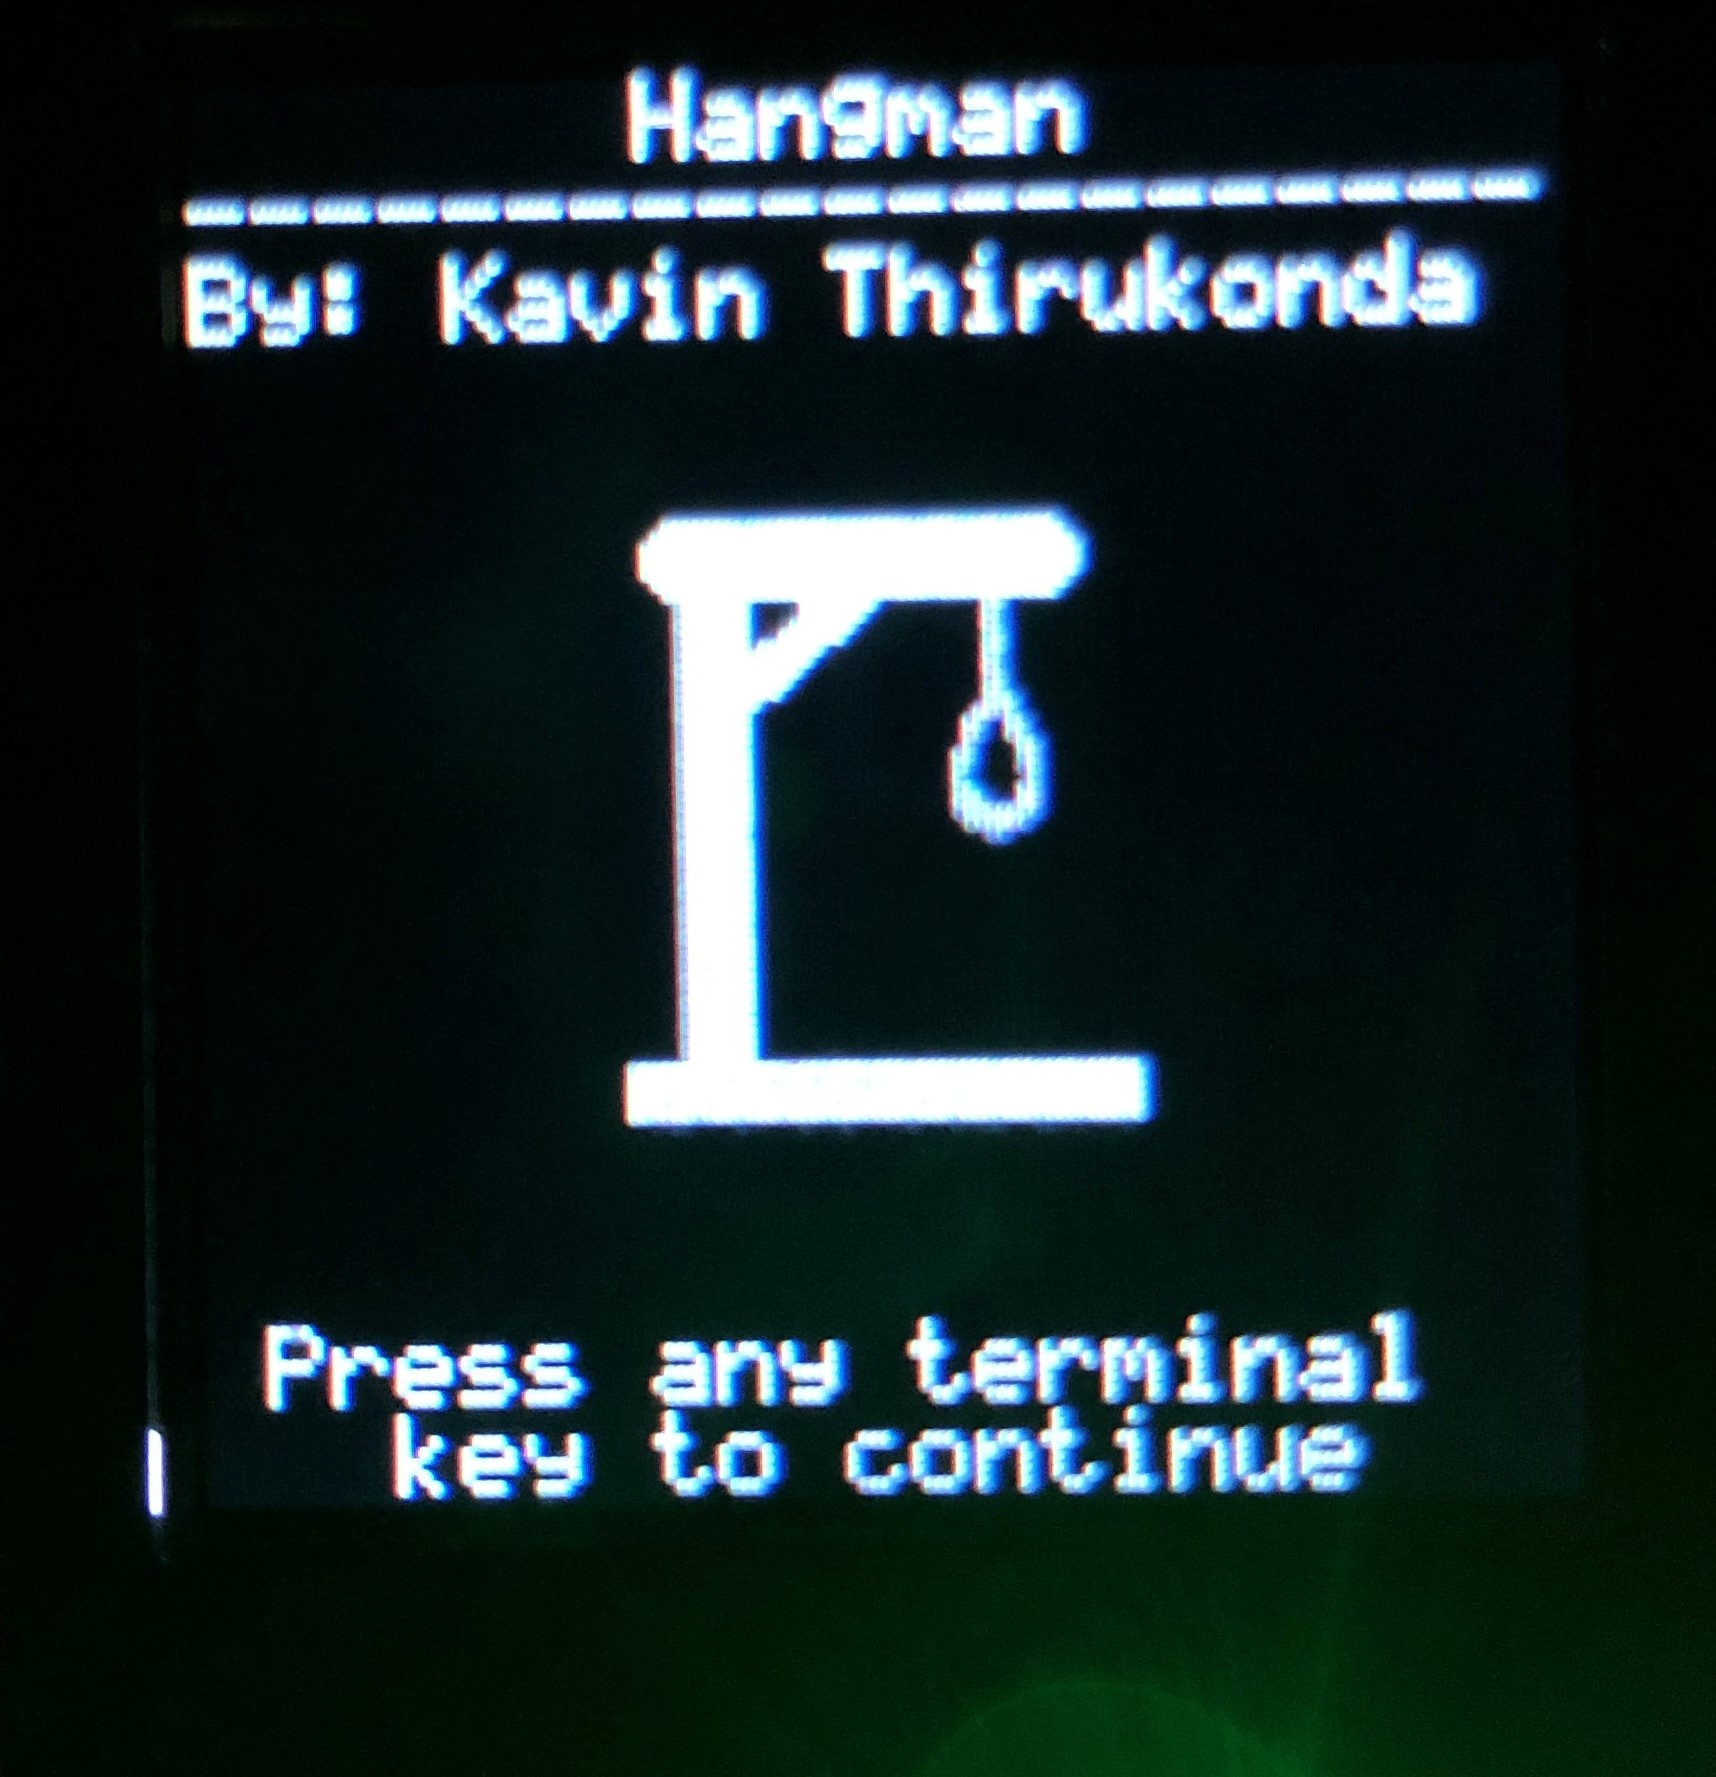
\includegraphics[width=.225\textwidth]{title.png}}
    \boxed{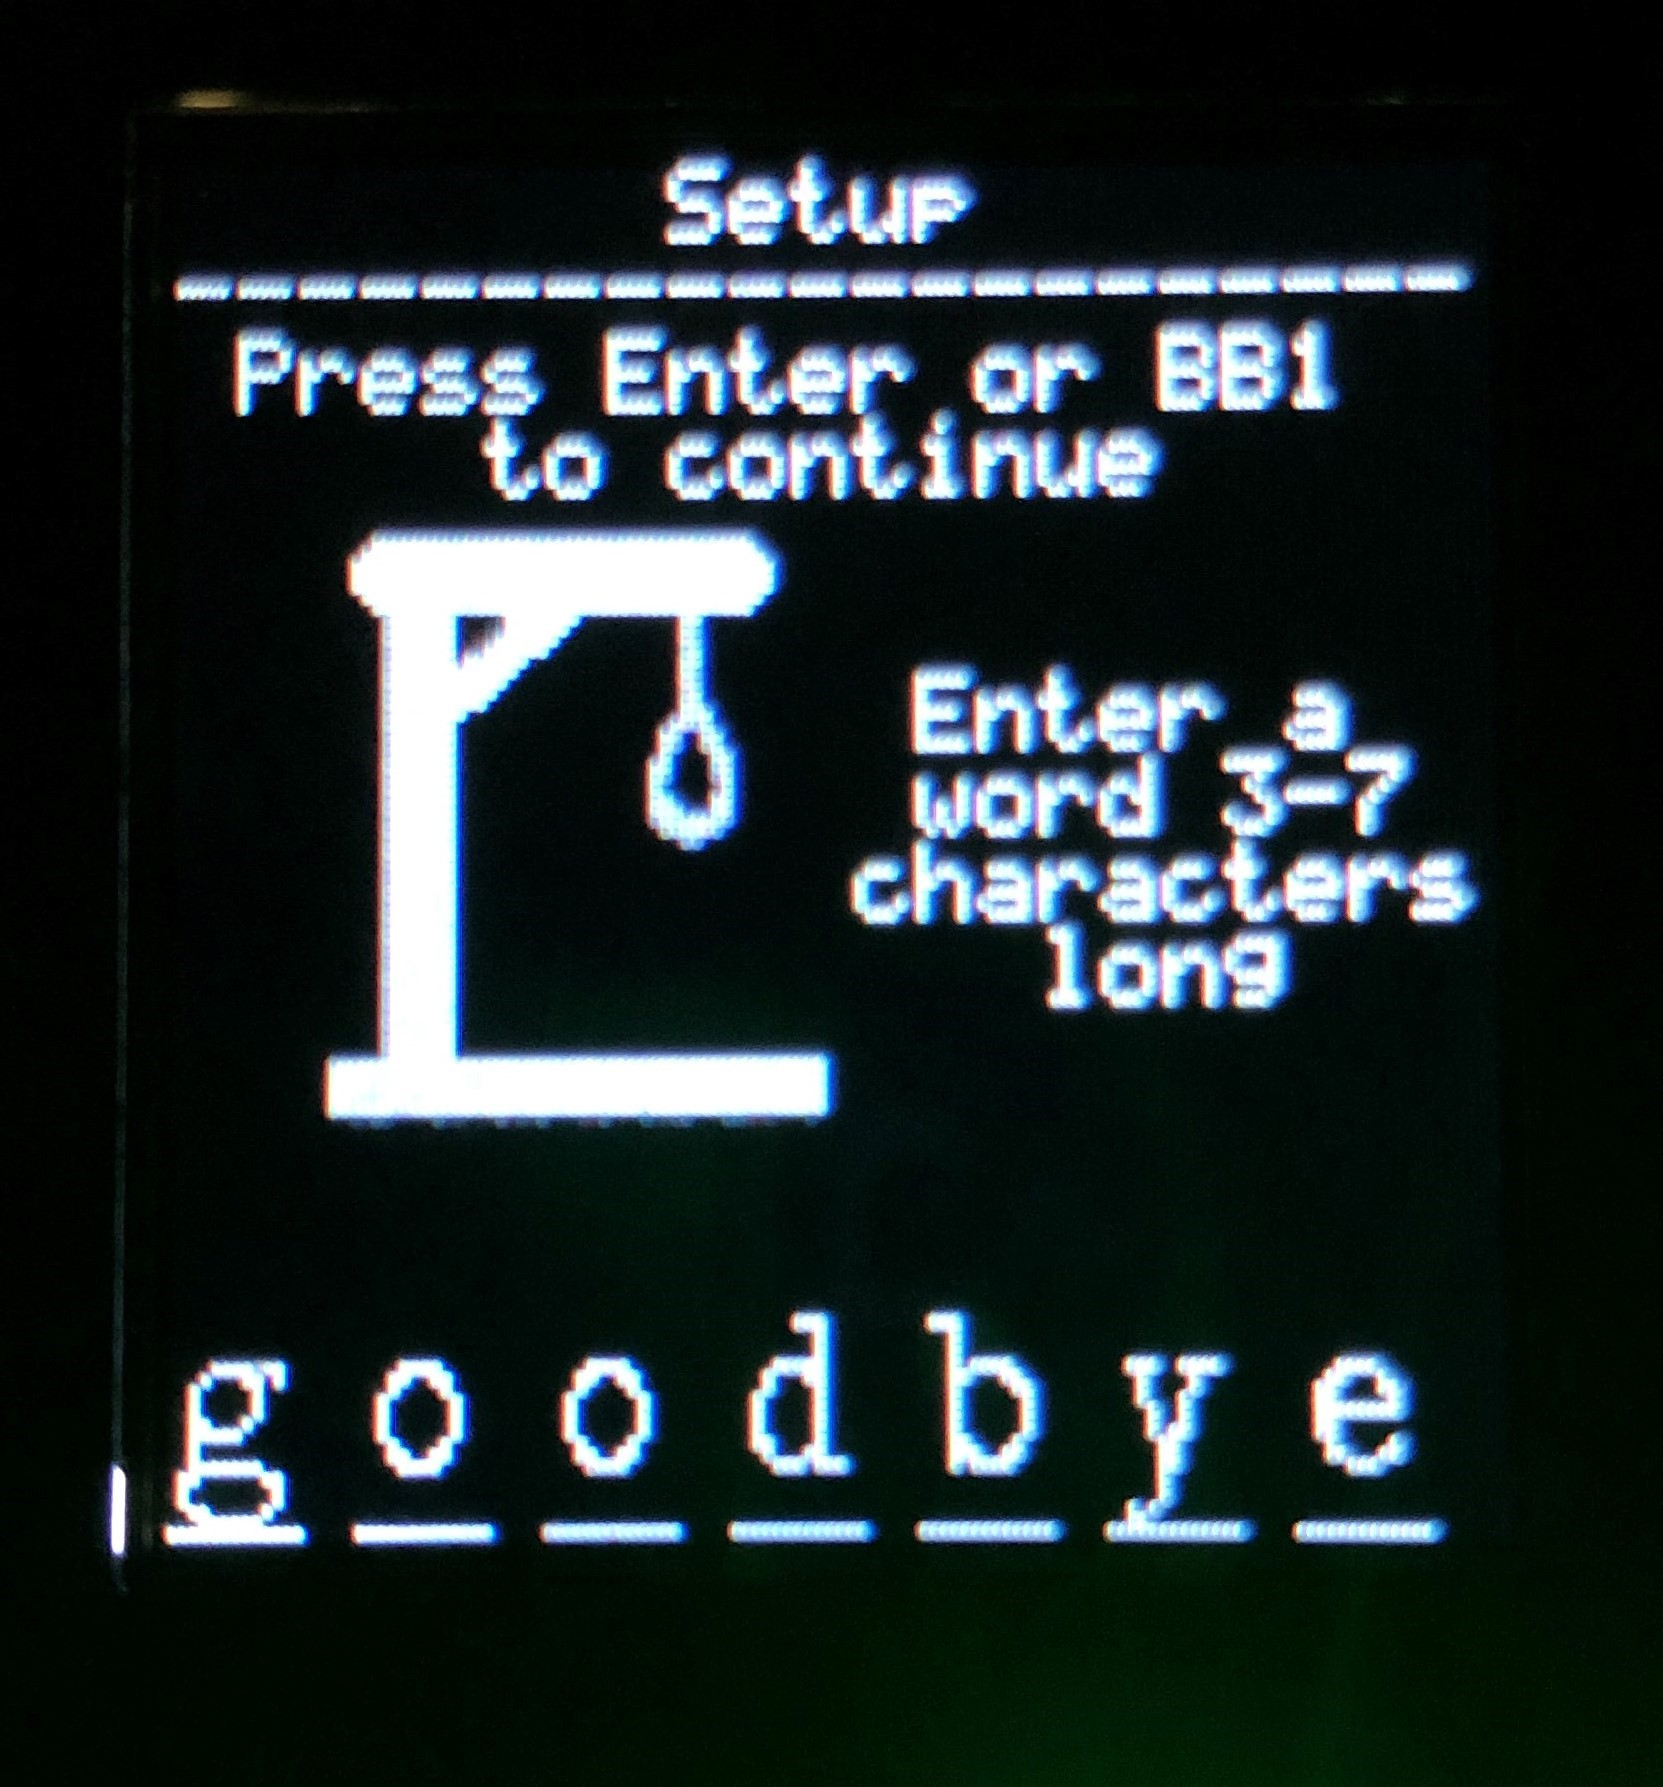
\includegraphics[width=.215\textwidth]{setup.png}}
    \boxed{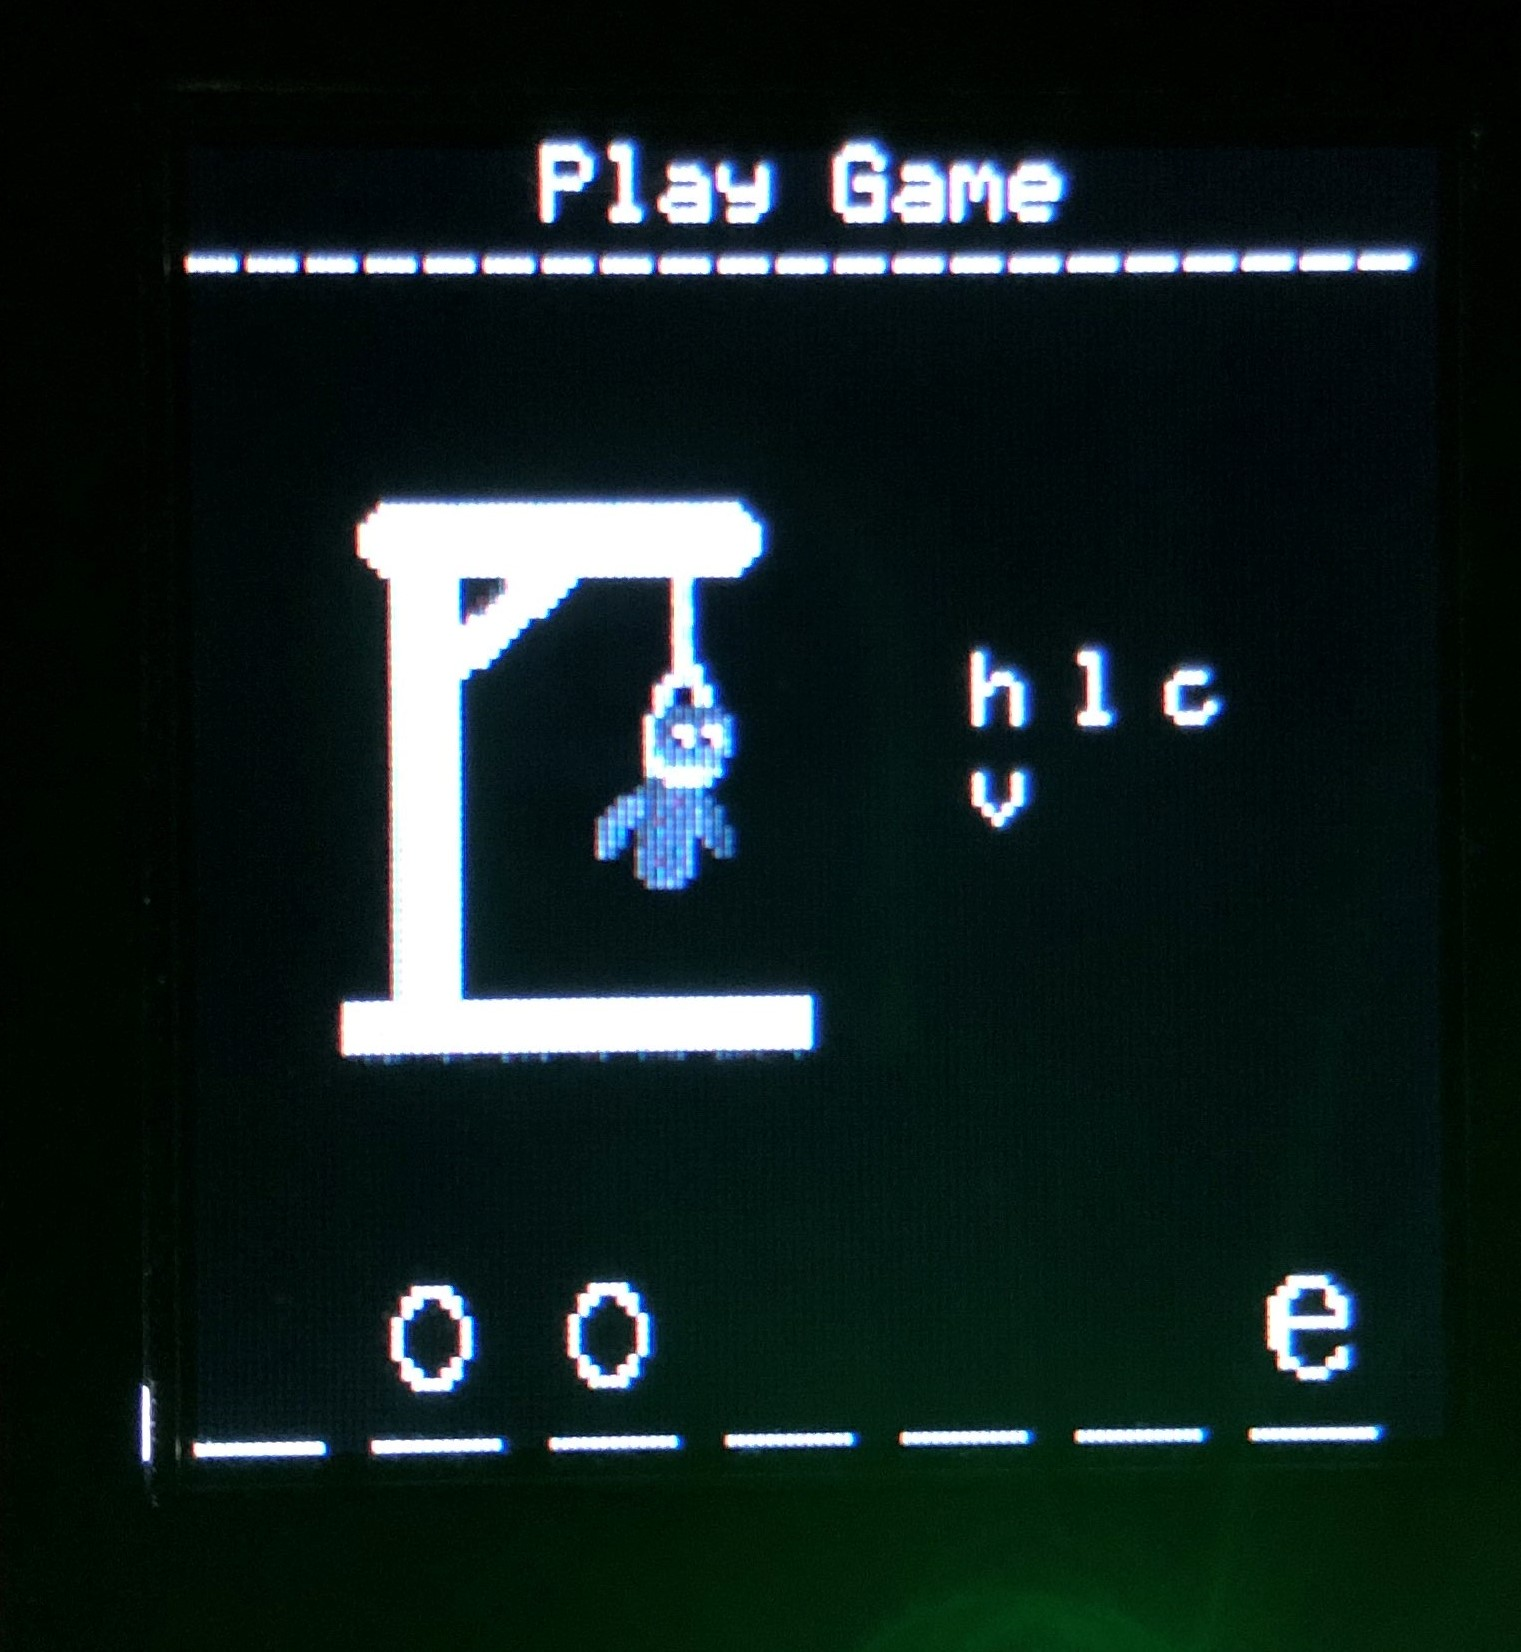
\includegraphics[width=.215\textwidth]{play.png}}
    \boxed{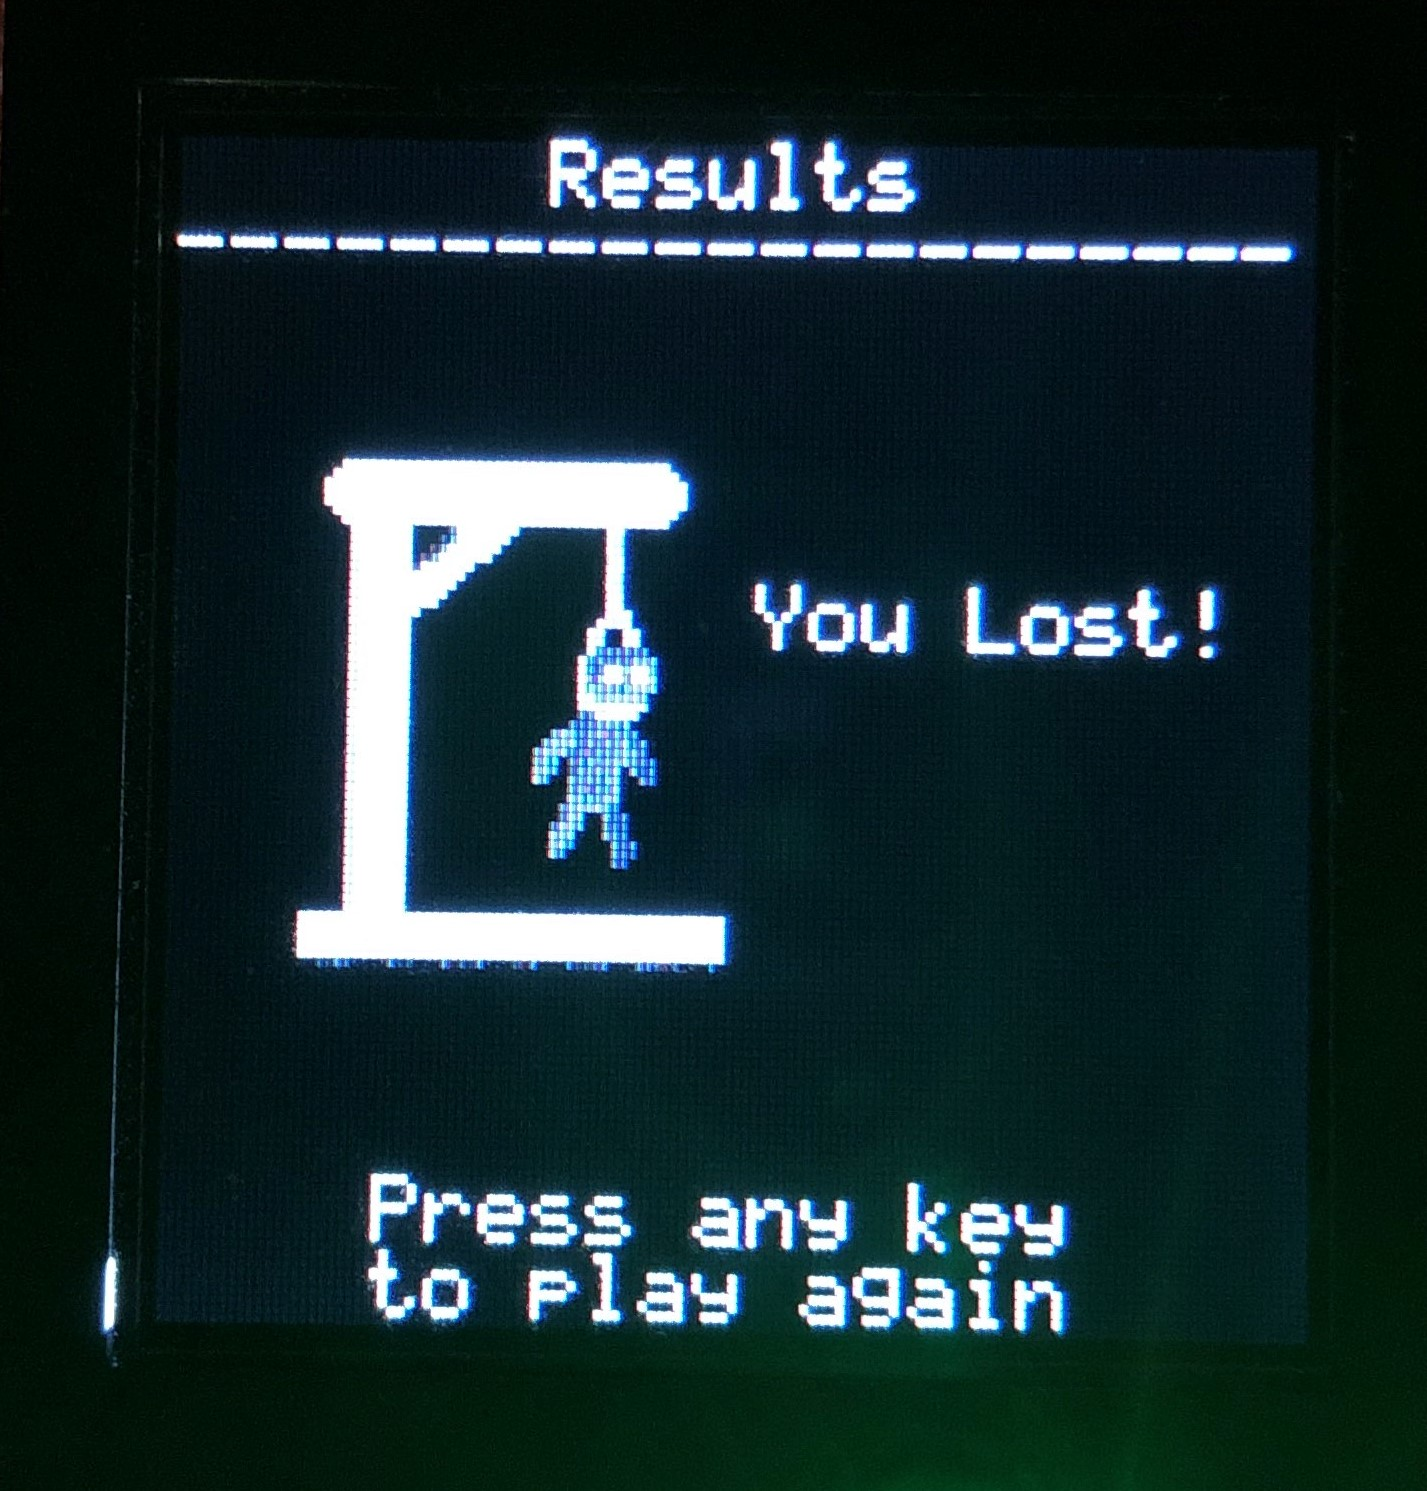
\includegraphics[width=.225\textwidth]{result.png}}
\end{center}

\section{Microcontroller-based embedded system architecture}
\begin{center}
    \begin{circuitikz}
    \draw (-2,0) node[draw,fill=pink,minimum width=40pt,minimum height=40pt](cpu){CPU}
    (-6,0) node[draw,fill=pink,minimum width=40pt,minimum height=40pt](msp){MSP}
    node[fit={(-3,-3)(3,3)},label={chip-level architecture},draw,inner sep=15pt]{}
    (-2,-2.5) node[draw,fill=pink,minimum size= 22.5pt](io1){I/O}
    (-1,-2.5) node[draw,fill=pink,minimum size= 22.5pt](io2){I/O}
    (0,-2.5) node[draw,fill=pink,minimum size= 22.5pt](io3){I/O}
    (1,-2.5) node[draw,fill=pink,minimum size= 22.5pt](io4){I/O}
    (2,-2.5) node[draw,fill=pink,minimum size= 22.5pt](io5){I/O}
    (0,2.5) node[draw,fill=pink,minimum size= 22.5pt](io6){I/O}
    (2,2.5) node[draw,fill=pink,minimum size= 22.5pt](io7){I/O}
    (0,1) node[draw,fill=pink,minimum width=30pt,minimum height=30pt](rx){$\begin{array}{c}euSCI\\RX\end{array}$}
    (2,1) node[draw,fill=pink,minimum width=30pt,minimum height=30pt](tx){$\begin{array}{c}euSCI\\TX\end{array}$}
    (cpu) to [short](io1)
    ($(cpu)+(.1,-.7)$) to [short]($(cpu)+(.1,-2)$)[short] to [short]($(cpu)+(1,-2)$)to[short]($(io2)+(0,.4)$)
    ($(cpu)+(.2,-.7)$) to [short]($(cpu)+(.2,-1.9)$)[short] to [short]($(cpu)+(2,-1.9)$)to[short]($(io3)+(0,.4)$)
    ($(cpu)+(.3,-.7)$) to [short]($(cpu)+(.3,-1.8)$)[short] to [short]($(cpu)+(3,-1.8)$)to[short]($(io4)+(0,.4)$)
    ($(cpu)+(.4,-.7)$) to [short]($(cpu)+(.4,-1.7)$)[short] to [short]($(cpu)+(4,-1.7)$)to[short]($(io5)+(0,.4)$)
    (io1) to [short,-*] ($(io1)+(0,-1.03)$) node[anchor=north]{P1.0}
    (io2) to [short,-*] ($(io2)+(0,-1.03)$) node[anchor=north]{P1.1}
    (io3) to [short,-*] ($(io3)+(0,-1.03)$) node[anchor=north]{P1.2}
    (io4) to [short,-*] ($(io4)+(0,-1.03)$) node[anchor=north]{P3.5}
    (io5) to [short,-*] ($(io5)+(0,-1.03)$) node[anchor=north]{P2.0}
    ($(rx)+(0,-.55)$) to [short]($(cpu)+(2,0)$) to [short](cpu)
    ($(tx)+(0,-.55)$) to [short]($(cpu)+(4,-.1)$) to [short]($(cpu)+(.71,-.1)$)
    (io6) to[short](rx)
    (io7) to[short](tx)
    ($(io6)+(0,.4)$) to [short]($(io6)+(0,.8)$) to [short,-*]($(io6)+(3.53,.8)$)node[anchor=west]{P1.3}
    ($(io7)+(0,.4)$) to [short]($(io7)+(0,.5)$) to [short,-*]($(io7)+(1.53,.5)$)node[anchor=west]{P1.2}
    node[fit={(-11,-3)(-5,3)},label={board-level architecture},draw,inner sep=15pt]{}
    (-6,2)node[draw,circle,fill=pink](ll1){LL1}
    (-7.25,2)node[draw,circle,fill=pink](ll2){LL2}
    (-8.5,2)node[draw,circle,fill=pink](bb1){BB1}
    (-9.75,2)node[draw,circle,fill=pink](bb2){BB2}
    (-6,-3.5)node[draw,fill=pink,minimum width=20pt,minimum height=20pt](usb){USB} to [short]
    (-6,-2.5)node[draw,fill=pink,minimum width=20pt,minimum height=20pt](xds){XDS} to [short]
    (-6,-1.5)node[draw,fill=pink,minimum width=20pt,minimum height=20pt](iso){Isolation}
    (msp) to [short] (ll1);
    \draw ($(iso)+(.2,.34)$) to [short]($(iso)+(.2,.78)$);
    \draw ($(iso)+(-.2,.34)$) to [short]($(iso)+(-.2,.78)$);
    \draw ($(msp)+(-.1,.7)$) to [short]($(msp)+(-.1,1.4)$) to [short]($(msp)+(-1.25,1.4)$) to [short]($(msp)+(-1.25,1.5)$);
    \draw ($(msp)+(-.2,.7)$) to [short]($(msp)+(-.2,1.3)$) to [short]($(msp)+(-2.5,1.3)$) to [short]($(msp)+(-2.5,1.5)$);
    \draw ($(msp)+(-.3,.7)$) to [short]($(msp)+(-.3,1.2)$) to [short]($(msp)+(-3.75,1.2)$) to [short]($(msp)+(-3.75,1.5)$);
    \draw (-10,0) node[draw,fill=pink,minimum width=35pt,minimum height=35pt](lcd){LCD} to[short](msp);
    \end{circuitikz}
\end{center}
\begin{center}
    Assuming the two boards we have are one, the architecture of this system is quite simple, since a very low amount of inputs from the actual boards are used, most inputs come from the UART terminal, this goes through a USB, into the XDS, and into an isolation circuit which then both get fed into the chip and processed from there and that's most of the inputs there.
\end{center}
\newpage
\section{Code Quality}
\subsection{Comments}
\begin{center}
    The comments in my code show what each function does, the input and output of each function, and whenever a chunk of code is called there is a brief explanation of when the code will be called and what happens when the code does get called. 
\end{center}
\subsection{No Global Variables}
\begin{center}
    The only global variables used are the ones used for images which according to specification are allowed
\end{center}
\subsection{No Numeric Values}
\begin{center}
    all values are defined using macros, which explain the meaning of the number
\end{center}
\subsection{No Long Functions}
\begin{center}
    All functions are below max length and line number commented at the top of relevant functions.
\end{center}
\subsection{Using HAL} 
\begin{center}
    The HAL were used properly when needed.
\end{center}
\subsection{Non-Blocking Code}
\begin{center}
    In all places of the code the blocking test did in fact turn on the LED and therefore the code is nonblocking.
\end{center}
\begin{center}
    \begin{tabular}{c|c}
         Code Quality Aspect &  Expected Points\\
         \hline
         Comments & 10\\
         No Global Variables & 20\\
         No Numeric Values & 20\\
         No Long Functions & 30\\
         Non-Blocking Code & 20\\
    \end{tabular}
\end{center}
\newpage
\section{Bonus Points}
\begin{center}
    Write one or more paragraphs explaining which bonus features your application achieves (if any), and how you implemented those. Create a table or bulleted list with the features you have implemented and the number of points you expect to get from those bonus features. Add a row (or bullet) for the total points you expect to get from bonus points.
\end{center}
\subsection{Difficulty Levels}
\begin{center}
    Implemented all required difficulty levels plus one extra difficulty, in which the guesser only has one guess to get the entire word.
\end{center}
\subsection{Custom title/result screen}
\begin{center}
    Both a custom title screen and a custom results screen in the title screen the gallows are shown empty, and on the result screen the hangman is shown based on how many missed guesses there are, and if the game is lost the hangman is shown dead.
\end{center}
\subsection{Custom hangman}
\begin{center}
    I drew a custom hangman with some nice shading he is a rock man and his name is brad, sadly brad needs to die over and over for the sake of my grade.
\end{center}
\subsection{Backspace}
\begin{center}
    Implemented back space, gets rid of both the letter and the underscore under the letter as I chose to draw underscores in the setup screen.
\end{center}
\subsection{Feedback}
\begin{center}
    The feedback is implemented according to spec if enter is pressed before 3 letters are entered, the screen is cleared and a prompt to enter a word in the correct range is shown.
\end{center}
\begin{center}
    \begin{tabular}{c|c}
         Bonus Opportunities &  Expected Points\\
         \hline
         Difficulty Levels & 50\\
         Custom title/result screen & 20\\
         Custom hangman & 50\\
         Backspace & 50\\
         Feedback & 50\\
    \end{tabular}
\end{center}
\end{document}
